The concept of barrier coverage \cite{kumar2005barrier}, was first introduced specifically for intruder detection applications in WSNs where sensing regions of sensor nodes form one or multiple barriers so that any intruder penetrating the region of interest will be detected. Due to its superiorities for security applications, barrier coverage has received attentions in recent years. The barrier coverage problems in WSNs can be categorized into two sub-problems: one is finding penetration paths. A penetration path is continuous curve with arbitrary shape, go though one side to the other side of a sensor field; other is building intrusion barrier for detecting intrusion of a mobile object when it traverse from on side to the other side of the sensing field. The first problems have thoroughly been delved into many researches such as \cite{megerian2002exposure,binh2016heuristic,liu2013percolation,binh2017genetic,binh2019efficient}, the second ones mostly focused on critical condition analysis (e.g., sensor node density) and barrier construction for stationary sensors with omni-directional sensing coverage models. \cite{liu2008strong,saipulla2008barrier,he2010distributed,skraba2007energy,chen2013energy}. Directional sensing coverage models then were widely used such as camera, radar etc., and taken into consideration in coverage problems as well as in barrier coverage problems.
 \cite{ai2006coverage,akyildiz2007survey,guvensan2011coverage,ma2005coverage,soro2005coverage}. Barrier coverage problems in WCSNs are much more complexed and challenging compared to those in traditional scalar WSNs \cite{chang2006collaborative,ma2012minimum,makhoul2009adaptive,wang2011barrier}, because of WCSNs having unique features.
 
 The authors \cite{chang2006collaborative} proposed a collaborative technique for face
 analysis in WCSNs with a dual objective of
 detecting the camera view closest to a frontal view of the
 object, and assessing angles between the face directional and all the camera views based on additional fusion of local angle estimates. To gather more information of the stable object, especially face recognition, full-view coverage was introduced in \cite{wang2013achieving} by Wang et al. An object is full-view covered if its face is always a camera to cover it no matter which face direction and the angle between the camera’s viewing direction and the object’s facing direction is less than a predefined parameter $\theta$. The authors proposed a method for full-view coverage verification on a sensing field. After that, they derived an estimation of the sensor density needed for full-view coverage in a random deployment. Based on this work, Wang et al. further studied the problem of constructing a camera barrier in \cite{wang2011barrier}. They proposed a method to select camera sensors from an arbitrary deployment to form a camera barrier and then presented a technique for reducing the number of cameras used since there might be redundant cameras (cameras that can be turned off without breaking the barrier) after barrier is formed.
 Besides, Ma et al. \cite{ma2012minimum}, proposed a better method for constructing camera barrier. With aiming at minimum the number of camera sensors in full-view barrier coverage, the problem is transformed into the shortest path problem from the source to the destination node on graph. \textcolor{ProcessBlue}{\bfseries However, the algorithm using in this work cannot be used to solve the problem}. This algorithm can be considered as a variant of Dijkstra algorithm. The only two differences are: (1) the edge has no weight but each vertex $v$ has a "weight" denoted by $I(v)$ and (2) the operator used for updating label of a vertex is union instead of addition. The second difference is the reason why the algorithm has problem. According to the algorithm, when a vertex $v$ is labeled, every previous vertex in the path from source vertex $s$ to $v$ is also labeled. Supposed $u$ is such a vertex between $s$ and $v$, the shortest path from $s$ to $u$ must be contained in the path from $s$ to $v$. But this is not true when the operator union is used, Figure \ref{fig:01} illustrates this.
 
\begin{figure}[p]
	\centering
	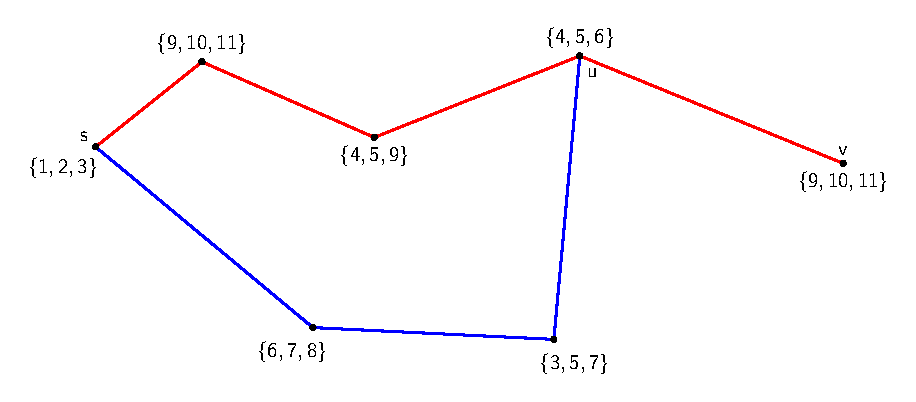
\includegraphics[scale=0.6]{wrongDijstra.pdf}
	\caption{Red line is shortest path from $s$ to $v$. Blue line is shortest path from $s$ to $u$}
	\label{fig:01}
\end{figure}

To monitor the object from multiple perspectives, Tseng et al. \cite{tseng2012k} introduced the notion of $k$-angle coverage. To avoid duplicating information from multiple sensors simultaneously monitoring an object, an angle constraint was added, which guaranteed  any two sensors cannot appear in an angle range of $\omega$ around the object (Figure \ref{fig:02}). It was pointed out that if an object is $(k-\omega)$ angle covered, there is no angle larger than $2\pi-(k-1)\omega$ of the object that is not covered by any sensor. This means that an object that is $(k-\omega)$ angle covered is also full-view covered with parameter $\theta=\displaystyle\frac{2\pi-(k-1)\omega}{2}$. Hence, $(k-\omega)$ angle coverage can be considered as a special case of full-view coverage with the number of camera sensors covering the object is fixed. Under this new coverage model, the paper focused on maximizing number of static objects that are covered using minimum number of sensors.
\begin{figure}[p]
	\centering
	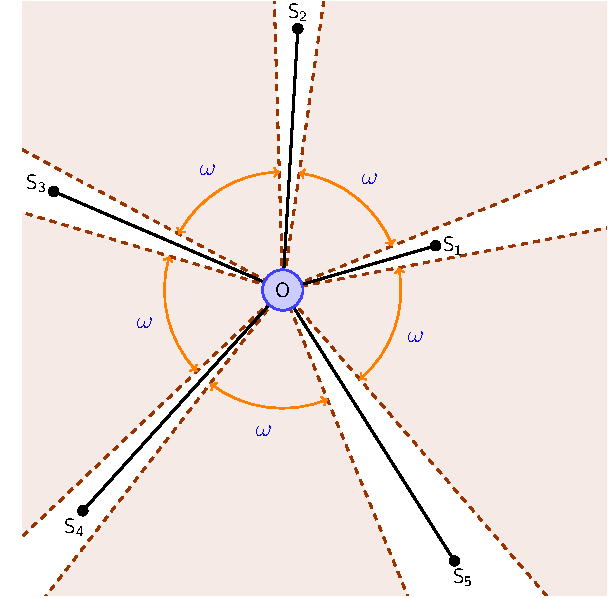
\includegraphics[scale=0.6]{komega.pdf}
	\caption{$O$ is 5-$\omega$-angle covered by $\{S_1, S_2, S_3, S_4, S_5\}$}
	\label{fig:02}
\end{figure}

In \cite{xu2016minimum}, the authors studied the problem of constructing $(k-\omega)$-angle barrier using minimum number of sensors called MkABC. The paper presented MkABC problem in two sensor deployment schemes. Under deterministic deployment, a geometric method was proposed, which used the feature of regular polygon to construct a ($k-\displaystyle\frac{\pi}{k}$)-angle barrier. When sensors are randomly deployed in the ROI, the MkABC becomes more difficult. In this scenario, the authors proposed a grid-based method, where each grid is judged to be $(k-\omega)$-angle covered or not. MkABC problem is then transformed into the shortest path problem on graph. The algorithm used is the same as one used in \cite{ma2012minimum}, which has some problems as aforementioned. Besides, The grid-based method has a trade-off between solution accuracy and the computational cost, which all depend on grid size chosen. This is a big disadvantage of this approach in large-scale WSN. 

Chen et al. \cite{chen2008measuring} first mentioned the problem of measuring the quality of barrier coverage in ODSNs. The authors introduced the notion of $L$-local $k$-barrier coverage to measure the quality of $k$-barrier coverage for a belt region as the maximum value of $L$ that the belt is $L$-local $k$-barrier covered. A belt region is said to be $L$-local $k$-barrier covered if every zone of length $L$ in the region is $k$-barrier covered. The measure always provides the same result when sensor network has already achieved k-barrier coverage, i.e, the probability of detecting the intruder by $k$ sensors is always 100\% which is equivalent to measuring its quality as 1 else zero, is not enough since there might be many different levels of quality coverage of the sensor barrier.  In addition, the considered k-barrier is just combination of consecutive sensing range. Actually, these metrics reflect constructing level of k-barrier, i.e. the closer distance L and the length of the strip region is, the more ROI achieves k-barrier. In contrast, our purpose evaluates quality of collected information in camera sensor barriers. This prompts us to devise a novel metrics called Differential coverage.  

%After considering many related works, we see that previous researches about barrier coverage problems in WCSNs are not yet efficient and there are rooms for improvement. Basing on $(k-\omega)$-angle coverage model \cite{xu2016minimum} with some fine-tuned for adapting to monitor mobile objects in barrier coverage in WCSNs, which refers to multiple view coverage model. Therefore, we produce the multiple view barrier coverage problem in WCSNs, then propose method as \textcolor{ProcessBlue}{\bfseries Dynamic Partition} to solve this problem. Furthermore, we desire to measure the quality of object's information recorded by sensors network when it crosses the barrier. Since the metrics proposed in \cite{chen2008measuring} is for $k$-barrier coverage model in ODSNs, it cannot apply to our problem. Moreover, this metrics only works when sensors network has not provided $k$-barrier coverage yet. In contrast, we need a metrics for measuring quality coverage of the barrier, which means the barrier must have been already constructed. These have fostered us to devise a new metrics called \textcolor{ProcessBlue}{\bfseries Differentiation Exposure}.


